
The script that solves the problem is \ttt{laplace.m} and is available at the end of the report with the subroutine \ttt{sol.m}. The boundary conditions in equation~\eqref{eq:cond2} are treated with ghost points. The conditions that the ghost point has the same value as the last point in the \textit{interior} of the domain. This is given by the discrete first derivative set to zero. We have numbered our unknowns vertically on the grid so that the band size is $M+2$ which is smaller than $N$ (the band we obtain when numbering the unknowns horizontally).

Here is the output of our script. With figures~\ref{fig:h02} and~\ref{fig:h01}.

\begin{lstlisting}
>> laplace
T(2,1) = 450.0000000000003979 for h = 0.2 
T(2,1) = 449.9999999999993747 for h = 0.1 
\end{lstlisting}

\begin{figure}[!h]
\centering
\includegraphics[width = 0.7\textwidth]{./h02.eps}
\caption{Solution with matlab for $h = 0.2$}
\label{fig:h02}
\end{figure}

\begin{figure}[!h]
\centering
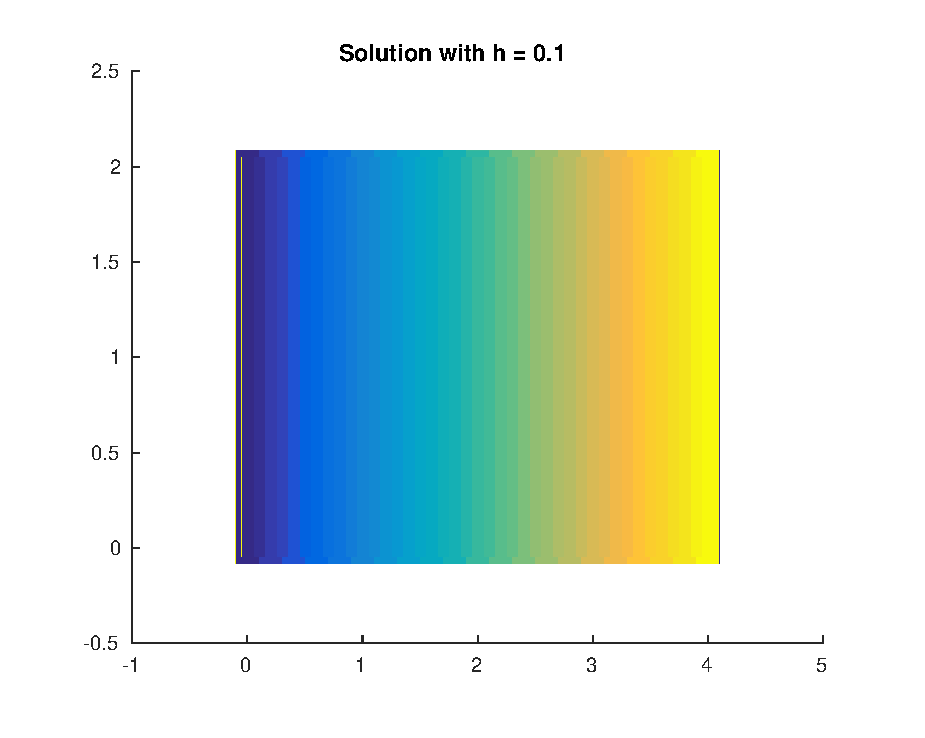
\includegraphics[width = 0.7\textwidth]{./h01.eps}
\caption{Solution with matlab for $h = 0.1$}
\label{fig:h01}
\end{figure}

\FloatBarrier

Let us assume that the solution $T(x,y)$ is independent of $y$ and is given by : 
$$T(x,y) = 300+75x$$

The Laplacian of this function $T$ is indeed zero everywhere inside the domain.

The boundary conditions $T(x=0)=300$ and $T(x=4)=600$ are satisfied. The solution respects also boundary conditions ~\eqref{eq:cond2}. By unicity (the problem is well posed), we can conclude that this is the solution.

 It is now clear that $T(2,1)=450$. The (notably small) errors in the numerical solution are \textit{only} due to floating point computation errors. Indeed, because the solution is linear, the finite differences give no longer an approximation of the Laplacian but the exact value. 
 
\begin{align*} 
 \Delta T &= \frac{T(x,y+h)+T(x,y-h)+T(x+h,y)+T(x-h,y)-4T(x,y)}{h^2}\\
 &=\frac{(300+75x)+(300+75x)+(300+75(x+h))+(300+75(x-h))-4*(300+75x)}{h^2}\\
 &=\frac{1200+300x+75h-1200-300x-75h}{h^2}\\
 &=0
 \end{align*}

This is also why the error is not reduced when decreasing $h$.